\documentclass[a4paper,
12pt,
BCOR12mm,
]{scrartcl}
%scrreport
\usepackage[ngerman]{babel}
\usepackage[utf8]{inputenc}
\usepackage[T1]{fontenc}
\usepackage{url}
\usepackage[pdftex]{graphicx}
\usepackage{listingsutf8}
\usepackage{grffile}
\usepackage{epstopdf}
\usepackage{subfigure}

% lstlisting settings
\lstset{
showspaces=false,
breaklines=true,
breakindent=0pt,
frame=single,
language=C,
extendedchars=true,
inputencoding=utf8/latin1,
identifierstyle=\ttfamily,
basicstyle=\tiny,
numbers=left,
numberstyle=\tiny,
label=nodeadlock1
}

\title{APUVS, Blatt 3}
\author{Jan Fajerski and Kai Warncke and Magnus Müller}

\begin{document}
% NOTE: compile with pdflatex --shell-escape main.tex

\maketitle  

\section{Verwendete Architekturen}
\subsubsection{Prozesse}
Der Großteil der Auswertung von \verb|fork()| erfolgte auf folgender Maschine:
\begin{verbatim}
% uname -a
Linux centraldogma 2.6.35-ARCH #1 SMP PREEMPT Sat Oct 30 21:22:26 CEST 2010
	x86_64 Intel(R) Core(TM) i5 CPU M 520 @ 2.40GHz GenuineIntel GNU/Linux

% cat /proc/meminfo
MemTotal:        3848056 kB
MemFree:         1889880 kB
Buffers:          352748 kB
Cached:           541128 kB
[...]
\end{verbatim}
\subsubsection{POSIX-Thread}
Der Großteil der Auswertung von POSIX-Threads erfolgte auf folgender Maschine:
\begin{verbatim}
% uname -a
Linux Zero2 2.6.35-ARCH #1 SMP PREEMPT Sat Oct 30 21:22:26 CEST 2010 
x86_64 Intel(R) Core(TM)2 Duo CPU T9400 @ 2.53GHz GenuineIntel GNU/Linux

% cat /proc/meminfoi
MemTotal:        3948772 kB
MemFree:         3143348 kB
Buffers:           67712 kB
Cached:           425560 kB
[...]
\end{verbatim}


\section{Aufgabe 3.1}
\subsection{a)}
\subsubsection{Erzeugung von Prozessen}
\begin{figure}[h!]
	\begin{center}
		\subfigure[fork (), Kindprozesse warten in Endlosschleife mit sleep ()]{
			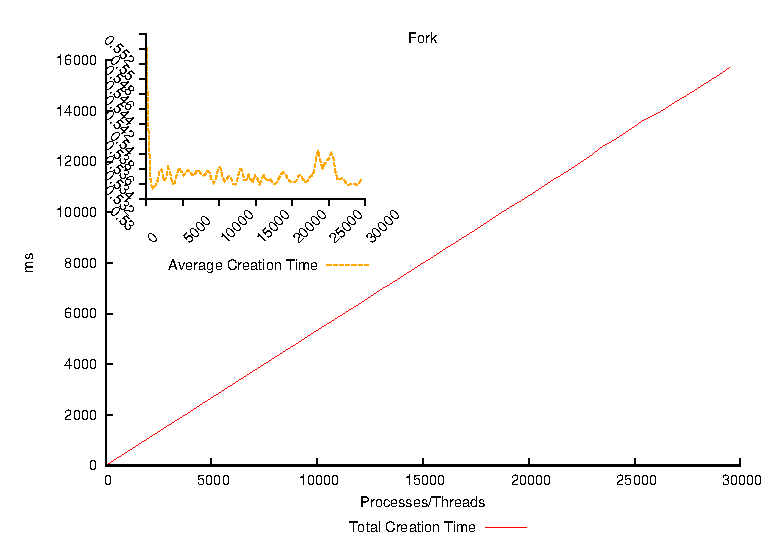
\includegraphics[scale=0.5]{../a_3_1/data/graphs/fork}
			\label{fig:fork_sleep}
		}
		\subfigure[fork () und exec ()]{
			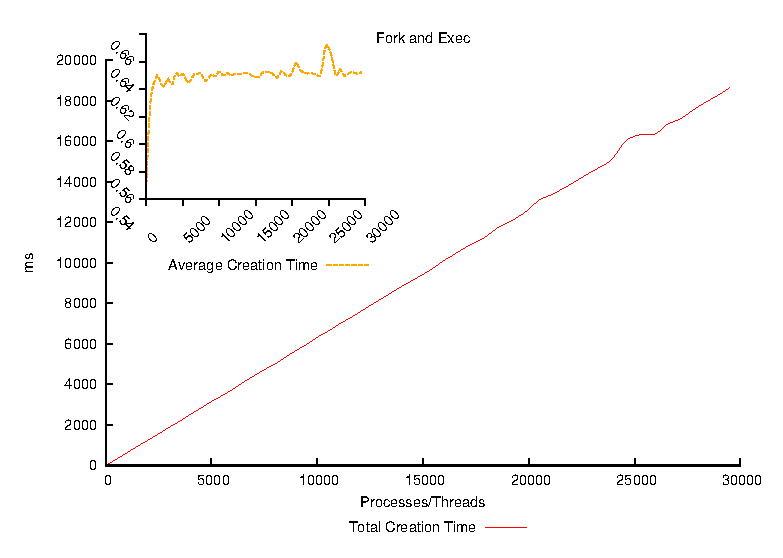
\includegraphics[scale=0.5]{../a_3_1/data/graphs/fork_exec}
			\label{fig:fork_exec}
		}
	\end{center}
\end{figure}

Wie an den Diagrammen \ref{fig:fork_sleep} und \ref{fig:fork_exec} zu erkennen ist,
benötigt die Erzeugung eines Prozesses per \verb|fork()| ca. $0.5$ms.
Hierbei ist zu beachten, dass \ref{fig:fork_exec} nur die Zeit zur Erstellung der Prozesse
misst, aber nicht die für \verb|exec()| benötigte Zeit. \\
Hieraus ergeben sich die Durchschnittswerte aus Tabelle \ref{fig:fork_mean}.
\begin{figure}[h!]
	\begin{center}
		\begin{tabular}[h!]{c|c}
			\hline
			fork & $0.534217$ms	 \\
			fork mit exec & $0.630396$ ms\\
			\hline
		\end{tabular}
	\end{center}
	\caption{Durchschnittswerte}
	\label{fig:fork_mean}
\end{figure}


\begin{figure}[h!]
	\begin{center}
		\lstinputlisting[ ] {../a_3_1/fork/max_processes.c}
	\end{center}
	\caption{Fork}
	\label{fig:fork_listing}
\end{figure}

\begin{figure}[h!]
	\begin{center}
		\lstinputlisting[ ] {../a_3_1/fork/max_processes_exec.c}
	\end{center}
	\caption{Fork mit exec}
	\label{fig:fork_exec_listing}
\end{figure}

\begin{figure}[h!]
	\begin{center}
		\lstinputlisting[ ] {../a_3_1/fork/messuretime.h}
	\end{center}
	\caption{Der header zur Zeitberechnung wird von allen fork Varianten eingebunden.}
	\label{fig:messuretime}
\end{figure}
\subsection{b)}
\subsubsection{Erzeugung von POSIX-Threads}
Um festzustellen wieviel Zeit die Erzeugung eines POSIX-Threads auf dem oben angegebenen System durchschnittlich
in Anspruch nimmt wurde dem Test-Programm max\_pthr 60 mal aufgerufen wobei die Anzahl zu erzeuegender Threads
jeweils um 500 erhöht wurde. Die ms/Thread wurden aufgezeichnet und führten zum folgenden Graphen.

%TODO: GRAPH max_pthr hier

Im Schnitt benötigt die Erzeugung eines POSIX-Threads 0.523893ms.

\subsection{Zusammenfassung}
% TODO add your stuff here
Offensichtlich benötigt die Erzeugung von Prozessen die meiste Zeit. Da bei
\verb|fork()| ein neuer Prozess durch komplette Kopie des bestehenden Prozesses
erzeugt wird, ergibt sich ein größerer Overhead als bei den anderen Varianten. Zwar
kann durch \emph{Copy-On-Write} einiges an Zeit eingespart werden (denn falls danach per
exec ein neues Programm in dem Prozess gestartet wird muss sowieso neu auf den Speicher
zugegriffen werden), doch bereits die Interaktion mit dem Kernel benötigt mehr Zeit als
bei Erzeugung von Threads mittels einer \emph{user-level threading library}.
\section{Aufgabe 3.2}
\subsubsection{a)}
\subsubsection{Prozesse}
Das Kommandozeilenwerkzeug \verb|ulimit| gibt die obere Grenze der maximalen Anzahl an
möglichen Nutzerprozessen an:
\begin{verbatim}
% ulimit -u
30030
\end{verbatim}
Dies wird auch durch die Grafik \ref{fig:fork_sleep} untermauert. Die zugrunde liegenden
Daten wurden durch ein Shellscript erbracht, welches das aus \ref{fig:fork_listing}
entstehende Programm mit einer wachsenden Zahl parametrisiert. Diese Zahl gibt an,
wieviele Prozesse durch das Programm gestarten werden sollen. Hierdurch ergab sich, dass
auf dem Testsystem auch die Erzeugung von fast $30000$ Prozessen keine merkliche
Verzögerung mit sich brachte.
\subsection{b)}
\subsubsection{Prozesse}
Der folgenden Betrachtung liegt der weiter unten gegebene Quelltext zugrunde.
\begin{figure}[h!]
	\begin{center}
		\subfigure[Kindprozesse arbeiten]{
			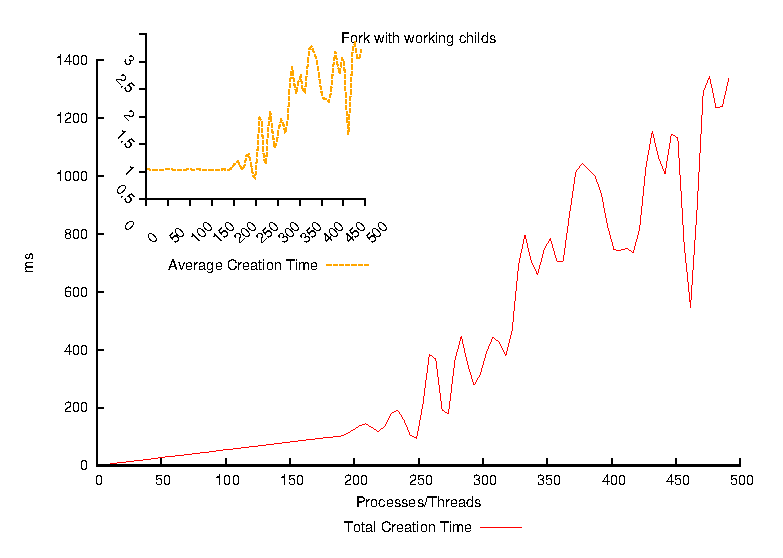
\includegraphics[scale=0.7]{../a_3_1/data/graphs/fork_childsworking}
			\label{fig:fork_childsworking}
		}
	\end{center}
\end{figure}
Erzeugt man eine Vielzahl (mehr als 200) von arbeitenden Kindprozessen, so kommt es unter Umständen zu
starkem \emph{thrashing}: die einzelnen Prozesse können zwar noch arbeiten, der großteil
der CPU-Zeit wird aber für Kontextwechsel verschwendet.\\
Dass dies mit der einfachen Berechenung der Prozesse auf der CPU zusammenhängt und nicht
nur mit dem Platzverbrauch der einzelnen Prozesse zeigt folgendes Beispiel:

\begin{verbatim}
% free -m && ./max_processes_childsworking 500 0 && free -m && pkill max_
             total       used       free     shared    buffers     cached
Mem:          3757       1943       1813          0        346        550
-/+ buffers/cache:       1047       2710
Swap:         8191          0       8191
Delta is: 1016.25000000
500 processes started 2.03250000 ms/Process
             total       used       free     shared    buffers     cached
Mem:          3757       1987       1770          0        346        550
-/+ buffers/cache:       1090       2667
Swap:         8191          0       8191
\end{verbatim}
Die 500 erzeugten Prozesse bringen keinen großen Platzverbrauch mit sich.
Interessanterweise benötigt aber die Erzeugung von Prozessen mehr Zeit als in Aufgabe
3.1a).
\begin{figure}[h!]
	\begin{center}
		\lstinputlisting[ ] {../a_3_1/fork/max_processes_childsworking.c}
	\end{center}
	\caption{Fork mit arbeitenden Kindprozessen}
	\label{fig:fork_childsworking_listing}
\end{figure}
\end{document}
